La différence entre les trois algorithmes étudiés se trouve dans la manière de conjuguer les volumes finis \cite{LeVeque1990} et la multirésolution adaptative.
Le paradigme des volumes finis nécessite le calcul d'un \textit{flux},
qui requiert lui l'évaluation de deux termes dépendant de la solution aux \textit{interfaces} amont et avales des cellules. À cellule $k$ fixée, ces termes sont notés $\Phi^+$ et $\Phi^-$.
Le problème est que les volumes finis n'approximent que les valeurs moyennes sur les cellules et non les valeurs ponctuelles aux interfaces, nécessaires au calcul des flux.
Les schéma volumes finis approximent alors les termes de flux comme fonction des valeurs moyennes sur les cellules voisines de l'interface.
À titre d'exemple, pour la diffusion, le flux en amont de la cellule $k$ est calculé comme $\frac{u_{k} - u_{k-1}}{\Delta x}$.\par
La MRA rend l'explication précédente non-univoque, la manière de calculer les flux peut être définie de plusieurs façon et c'est ceux en quoi les trois algorithmes étudiés diffèrent.\par 
Comme la MRA défini plusieurs grilles de pas $\Delta x,2 \Delta x, 4 \Delta x,...$ le choix de la grille sur laquelle choisir cellules voisines intervenant dans le calcul du flux est ambigu. 
En effet, à niveau de détail $l$ fixé, doit-ont évaluer les termes de flux à partir des cellules voisines du niveau $l,l+1,l+2...$ (voir le schéma en fig. \ref{fig:schema_algos}) ? 
Le premier algorithme étudié (la référence en MRA), consiste à évaluer les termes de flux à partir des voisins au même niveau que la cellule étudiée. C'est à dire que 
si la cellule est de niveau $l$, les voisines de l'interface sont choisit également au niveau $l$. Cela revient à résoudre localement l'EDP au niveau courant de la grille,
il est la norme en MRA car ne ne requiert aucun calcul supplémentaire, les valeurs sur la grille au niveau $l$ sont directement accessibles.
Le second algorithme consiste à systématiquement les valeurs de la grille la plus fine. Intuitivement c'est le plus précis, mais cela peut s'avérer très coûteux car 
la grille plus fine n'est pas directement accessible. Par exemple si la MRA à choisir une grille plus grossière de 4 niveau par rapport à la grille la plus fine, il 
faut reconstruire les valeurs au travers de 4 niveau. Enfin le troisième algorithme est un compromis entre les deux méthode précédents, il consiste à utiliser calculer les flux à partir des valeurs un niveau en deçà du niveau courant, pour gagner un peu en précision sans pour autant s'exposer à des coûts prohibitifs.
\begin{figure}[htpb]
\begin{center}
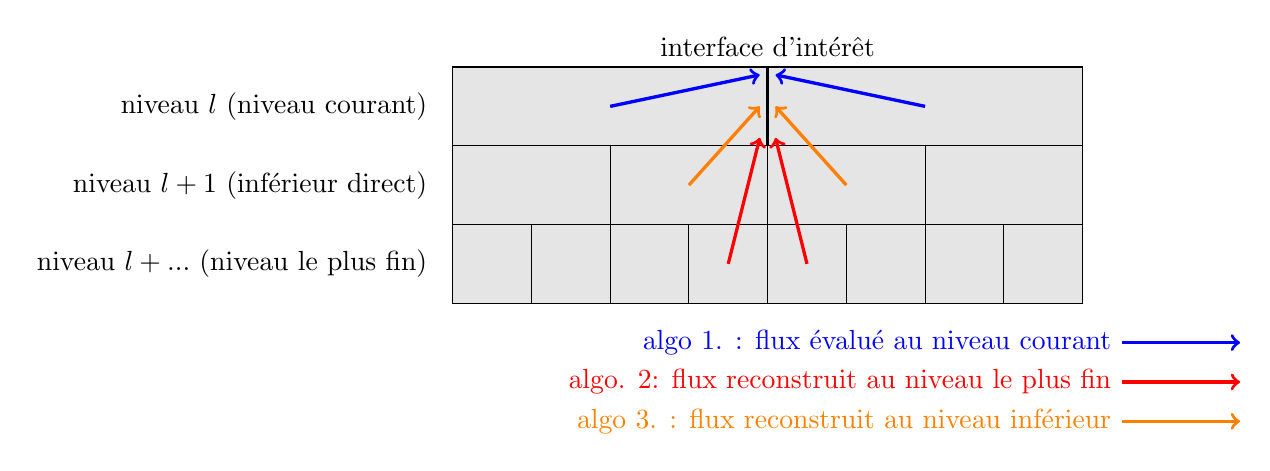
\begin{tikzpicture}
\foreach \i in {0,...,1}{
    \draw[fill=black!10] ({4*\i},0) rectangle ({4*(\i+1)},1);
}
\foreach \i in {0,...,3}{
    \draw[fill=black!10] ({2*\i},-1) rectangle ({2*(\i+1)},0);
}

\foreach \i in {0,...,7}{
    \draw[fill=black!10] ({\i},-2) rectangle ({(\i+1)},-1);
}

\draw[blue, very thick, <-] (3.9,.9) -- (2,.5);
\draw[blue, very thick, <-] (4.1,.9) -- (6,.5);

\draw[orange, very thick, <-] (3.9,.5) -- (3,-.5);
\draw[orange, very thick, <-] (4.1,.5) -- (5,-.5);

\draw[red, very thick, <-] (3.9,.1) -- (3.5,-1.5);
\draw[red, very thick, <-] (4.1,.1) -- (4.5,-1.5);

\draw[black, very thick] (4,0) -- (4,1) node[pos=1, above] {interface d'intérêt};
\node[left] at (-.2,.5) {niveau $l$ (niveau courant)};
\node[left] at (-.2,-.5) {niveau $l+1$ (inférieur direct)};
\node[left] at (-.2,-1.5) {niveau $l+...$ (niveau le plus fin)};

\draw[blue, very thick,->] (8.5,-2.5) -- (10,-2.5) node[pos=0,  left] {algo 1. : flux évalué au niveau courant};
\draw[red, very thick,->] (8.5,-3) -- (10,-3) node[pos=0,  left] {algo. 2: flux reconstruit au niveau le plus fin};
\draw[orange, very thick,->] (8.5,-3.5) -- (10,-3.5) node[pos=0,  left] {algo 3. : flux reconstruit au niveau inférieur};


\end{tikzpicture}
\caption{Illustration des trois algorithmes évalués. L'algorithme 1 en bleu calcul le flux à partir des cellule de la grille au même niveau que l'interface étudiée. 
L'algorithme 2 reconstruit les valeurs de la solution sur la grille de niveau inférieur. L'algorithme 3 reconstruit au niveau le plus fin possible. 
Plus l'algorithme reconstruit finement, plus les valeurs moyennes sont données sur des cellules petites et plus cela s'approche d'une valeur "ponctuelle".}
\label{fig:schema_algos}
\end{center}
\end{figure}